\documentclass{beamer}
\usecolortheme{wolverine}

% math stuff
\usepackage{amsmath}
\usepackage{amsthm}
\usepackage{amssymb}
\usepackage{xcolor}

\usepackage{float}
\usepackage{subcaption}

% to insert images
\usepackage{graphicx}

% to correctly insert stressed characters
\usepackage[T1]{fontenc}
\usepackage[utf8]{inputenc}

\usepackage{multirow}

% Bibliography
% \usepackage[style=alphabetic]{biblatex}
% \usepackage[nottoc]{tocbibind}
% \usepackage{bibentry}
% \setcounter{biburllcpenalty}{9000}
% \usepackage{nameref}
% \addbibresource{slides.bib}

% to put links in table of contents
\usepackage{hyperref}
\hypersetup{colorlinks=false, %set true if you want colored links
	linktoc=all,     %set to all if you
}

\usepackage{mathtools}

% Add symbols
% \usepackage{textcomp}

% Add command for Real and Z sets
% \usepackage{dsfont}
% \newcommand{\Rset}{$\mathds{R}$}
% \newcommand{\Zset}{$\mathds{Z}$}

% Code highlighting
% \usepackage{minted}
% \usemintedstyle{perldoc}
% \setminted{
%     frame=single,
%     breaklines,
% }

% tikz figures
% \usepackage{tikzit}
% \input{style.tikzstyles}

% number rounding
\usepackage{siunitx}
\sisetup{round-mode=places,round-precision=5}

\definecolor{myyellow}{RGB}{225, 225, 0}

\title{Thesis notes}
\date{4th May}

% any code between @(...)@ is escaped back to LaTeX
% \lstset{escapeinside={@(}{)@}}

% algorithms
\usepackage[ruled,vlined]{algorithm2e}
% \newtheorem{theorem}{Theorem}

\begin{document}

\frame{\titlepage}

\begin{frame}[c]
	\frametitle{The Echo Chamber Problem - notation}

	\begin{itemize}
		\item $G = (V, E ^{+}, E ^{-}) $ interaction graph
		\item $ \mathcal{C} $ set of contents
		\item $C \in \mathcal{C} $ content, $\mathcal{T} _{C} $ set of threads
		      associated with $C$. A thread $T \in \mathcal{T} _{C} $ is a
		      subgraph of $G$
		      % So $G = \bigcup _{C
		      % \in \mathcal{C} } \bigcup _{T \in \mathcal{T} _C} T $ union of all
		      % threads of all contents
		\item $U \subseteq V$ subset of users, $T[U]$ subgraph of $T$ induced
		      by $U$. $|T(U)|$ is the number of edges of this subgraph
	\end{itemize}
\end{frame}

\begin{frame}[c]
	\frametitle{The Echo Chamber Problem - notation}
	\begin{itemize}
		\item $\eta(C)$ fraction of negative edges associated with $C$
		      (analogous definition for a thread $T$). Content (or thread)
		      controversial if $\eta \in [\alpha, 1]$
		\item $\hat{\mathcal{C} } \subseteq \mathcal{C} $ set of \textit{controversial}
		      contents

		\item $\mathcal{S} _C (U)$ set of \textit{non controversial} threads
		      induced by $U$, for \textit{controversial} contents, i.e.

			      {\small
				      \begin{equation}
					      \mathcal{S} _{C} (U) = \{ T[U] \; s.t. \; T[U] \; non \;
					      controversial, T \in \mathcal{T} _{C}, C
					      \in \hat{\mathcal{C}}, U \subseteq V\}
				      \end{equation}
			      }
	\end{itemize}

\end{frame}

\begin{frame}[c]
	\frametitle{The Echo Chamber Problem}
	\textbf{Goal}: given an interaction graph $G$, find $U \subseteq V$ maximing

	\begin{equation}
		\xi (U) = \sum^{}_{C \in \hat{\mathcal{C}} } \sum^{}_{T[U] \in S_C (U)}
		| T[U] |
	\end{equation}

	The set of users maximing the expression is denoted as $\hat{U}$ and the
	corresponding score is $\xi(G)$
\end{frame}

\begin{frame}[c]
	\frametitle{The Densest Echo Chamber Problem}
	\textbf{Goal}: given an interaction graph $G$, find $U \subseteq V$ maximing

	\begin{equation}
		\psi (U) = \sum^{}_{C \in \hat{\mathcal{C}} } \sum^{}_{T[U] \in S_C (U)}
		\frac{| T[U] |}{|U|}
	\end{equation}

	The set of users maximing the expression is denoted as $\hat{U}$ and the
	corresponding score is $\psi(G)$
\end{frame}

\begin{frame}[c]
	\frametitle{A solvable Densest Echo Chamber problem (1)}

	Let $G = (V, E)$ be the interaction graph, $\delta(i, j)$ and $\delta^{-} (i, j)$ the sum of the
	edges and negative edges, respectively, between vertices $v_{i} $ and
	$v_{j} $ associated to controversial contents.

	\bigskip

	The graph $G_d = (V_{d}, E_{d}) $ is constructed as follows from G:

	\begin{itemize}
		\item for any vertex $v_{i} \in V$ add a corresponding vertex in $V_{d} $
		\item for any pair of vertices in $G $
		      \begin{itemize}
			      \item let $\eta(i,j) \coloneqq \frac{\delta^{-} (i,j)}{\delta
					            (i,j)} $. If $\eta(i,j) \leq \alpha $ add a positive
			            edge between $v_{i} $ and $v_{j} $ in $G_{d} $
			            % \item don't add any edge otherwise between $v_{i} $ and $v_{j} $
		      \end{itemize}
	\end{itemize}

	\paragraph{Densest non controversial subgraph}:%:
	\label{par:densest_non_controversial_subgraph}


	Let $E_{d} [U]$ the set of edges induced on $G_d$ by $U \subseteq V$. \textbf{Goal}: find $U$ maximizing

	\begin{equation}
		\xi(U) = \frac{|E_{d} [U]|}{|U|}
	\end{equation}

\end{frame}

\begin{frame}[c]
	\frametitle{A solvable Densest Echo Chamber problem (2)}
	Alternative taking into account threads:

	\begin{itemize}
		\item T-Densest non controversial subgraph: aggregate edges separately for each $T \in T_{C}, C \in
			      \hat{\mathcal{C}}$, i.e. let $\delta_{T}(i,j) $ be $\delta(i, j)$
		      for the subgraph $T$:
		      \begin{itemize}
			      \item let $\eta(T, i,j) \coloneqq \frac{\delta_{T} ^{-}
					            (i,j)}{\delta _{T} (i,j)} $. If $\eta(T, i,j) \leq \alpha
			            $ add a positive edge
		      \end{itemize}
	\end{itemize}

	Solve O$^{2} \textsc{Bff}$ problem on the preprocessed graph
	sequence, i.e.

	\bigskip

	\emph{Given a graph history $\mathcal{G}  = \{G_1 , G_2, . . . ,
			G_{\tau}  \}$, an aggregate density function $f$ , and an
		integer $k$, find a subset of nodes $S \subseteq V$ , and a
		subset $\mathcal{C} _{k} $ of $\mathcal{G} $ of size $k$,
		such that $f (S, C_k )$ is maximized}

	\bigskip

	O$^{2} \textsc{Bff}$-AM can be computed.
\end{frame}

\begin{frame}[c]
	\frametitle{Results}

	The algorithm (even if it is just an approximation) requires a lot of times
	even on smaller graphs.

	\bigskip

	For a graph with $100$ snapshots and $k = 10$, $|V| \approx 2000$ and $|E|
		\approx 2000$ it needs $> 6 $ hours.

\end{frame}

\begin{frame}[c]
	\frametitle{Results}

        \begin{figure}
        \begin{center}
            \begin{subfigure}[b]{0.4\textwidth}
                \centering
                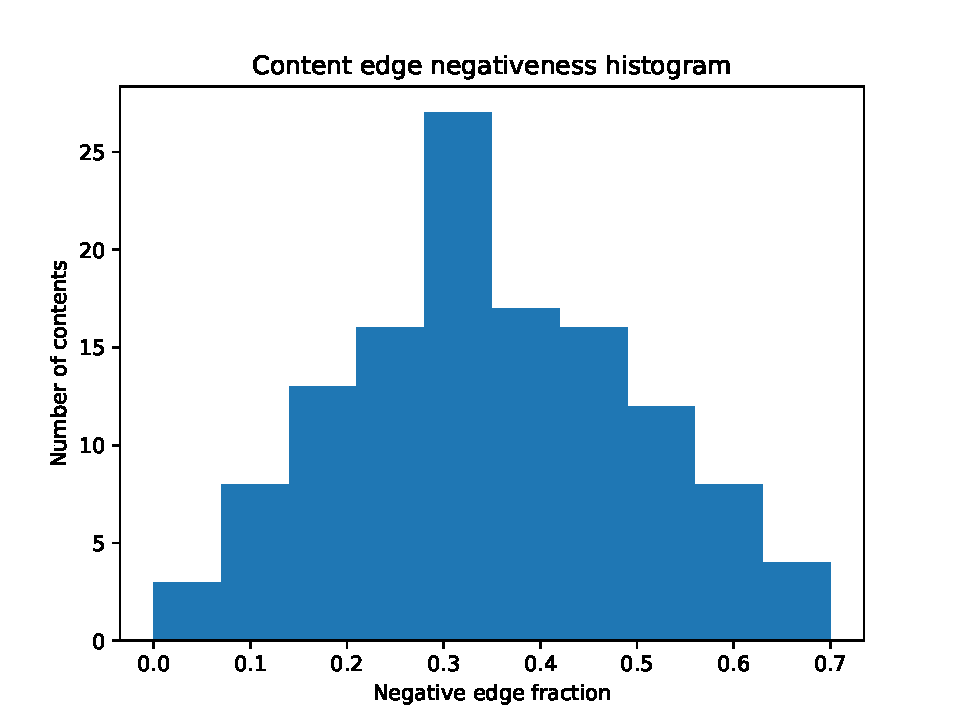
\includegraphics[width=\textwidth]{out/nytimes2000/neg-fraction-content-hist.pdf}
                \caption{@nytimes}
                \label{fig:nytimes-nef}
            \end{subfigure}
            \begin{subfigure}[b]{0.4\textwidth}
                \centering
                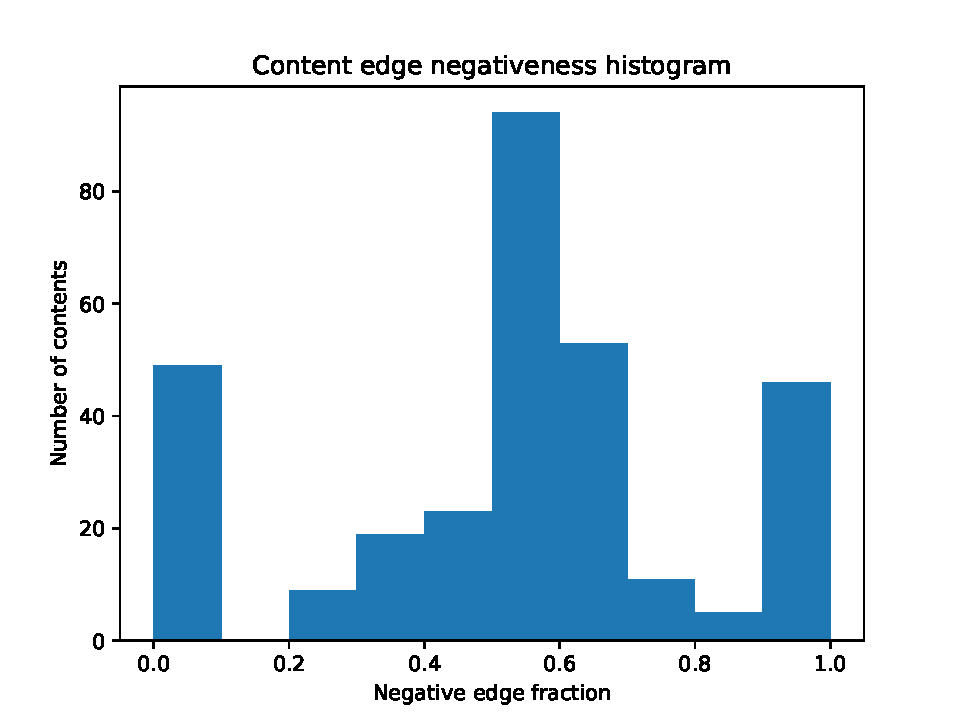
\includegraphics[width=\textwidth]{out/foxnews2000/neg-fraction-content-hist.pdf}
                \caption{@foxnews}
                \label{fig:out/foxnews2000/neg-fraction-content-hist.pdf}
            \end{subfigure}
        \end{center}
        \end{figure}
        

\end{frame}

\begin{frame}[c]
	\frametitle{Results}

	\tiny{
		\begin{table}[htpb]
			\centering
			\caption{Echo chamber scores. For the $\xi_{round}(G) $ the results tuple
				corresponds to (score, $|U|$, number of contributing threads, time in
				seconds). In the other scores the number of contributing thread
				is omitted. $\alpha = 0.4$}
			\begin{tabular}{c|c|c|c}
				\textbf{Source, $|V|$, $|E|$, $|\hat{\mathcal{C}}  |$} & $\xi_{round}(G) $          & $\psi_{Dens}(G)$ & $\psi_{T-Dest} (G)$ \\
				\hline
				nytimes, 20051, 24468, 44                                   &
                (5961, 4814, 243, 400)             & (1.2, 16, 1000)    &
                (1.2, 16, 1000)      \\
				foxnews, 45509, 82494, 232                                &
                (50240, 26352, 1090, 24000)          & (1.96, 28, 5000)    & (1.97,
                35, 5000)      \\
			\end{tabular}
		\end{table}
	}

	\tiny{
		\begin{table}[htpb]
			\centering
			\caption{Echo chamber scores for alpha chosen as the median of the
            $\eta$ of the contents. Tuple meaning is the same as above}
			\begin{tabular}{c|c|c|c}
				\textbf{Source, $|V|$, $|E|$, $|\hat{\mathcal{C}}  |$} & $\xi_{round}(G) $          & $\psi_{Dens}(G)$ & $\psi_{T-Dest} (G)$ \\
				\hline
				nytimes, 20051, 24468, 62                                   &
                (7337, 5775, 288, 243, 400)             & (1.2, 16, 1000)
                                                          & (1.2, 16, 1000)      \\
				foxnews, 45509, 82494, 154                                &
                (53643, 30816, 810, 24000)          & (1.96, 28, 5000)    & (1.97,
                35, 5000)      \\
			\end{tabular}
		\end{table}
	}

    \small{
    Median alpha for @nytimes: 0.358

    Median alpha for @foxnews: 0.553
    }
\end{frame}

\begin{frame}[c]
    \frametitle{Choosing alpha}
    It could be interesting to indagate the relationship between the Echo
    Chamber Score and alpha for different datasets, also relating it to the
    distribution of $\eta$ for the contents and threads.

    \begin{figure}[htpb]
        \centering
        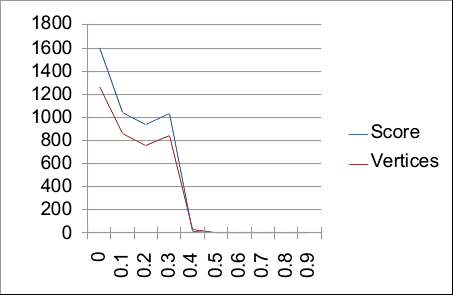
\includegraphics[width=0.6\linewidth]{img/cats_alpha_choice.png}
        \label{fig:img/cats_alpha_choice}
    \end{figure}
\end{frame}
% \begin{frame}[c]
%     \frametitle{A model for the Echo Chamber Problem (1)}
%     Model parameters:
%     \begin{itemize}
%         \item $b_{i} $, the group of each user $i$
%         \item $\omega ^{+} _{rs} $ and $\omega ^{-} _{rs} $, the probabilities
%               of positive and negative edges, respectively, between users in
%               group $r$ and $s$ ($\omega ^{+} _{rs} + \omega ^{-} _{rs} \leq 1$).
%         \item $\theta$, controlling the reduction of probability of interacting
%               between \emph{inactive} communities
%     \end{itemize}
%
%     For each content:
%     \begin{enumerate}
%         \item Sample $n'$ among the $n$ communities. These are the
%               \emph{active} communities in the content discussion
%         \item For each node pairing $i, j$ consider their corresponding groups $r$ and
%               $s$.
%               \begin{itemize}
%                   \item If both communities are \emph{active} draw from the
%                         categorical distribution $(\omega _{rs} ^{+}, \omega
%                             _{rs} ^{-}, 1 - \omega _{rs} ^{+} - \omega _{rs} ^{-}) $ to add an edge (or
%                         not).
%                   \item Otherwise draw from the categorical $(\theta \omega _{rs} ^{+},
%                             \theta \omega
%                             _{rs} ^{-}, 1 - \theta (\omega _{rs} ^{+} + \omega _{rs}
%                             ^{-}))$, $\theta \leq 1$.
%               \end{itemize}
%
%     \end{enumerate}
%
% \end{frame}

\begin{frame}[c]
	\frametitle{A model for the Echo Chamber Problem}
	Again each node has a group assignment and there are probabilities of
	positive and negative edges $\omega _{rs}^{+}  $ and $\omega _{rs}^{+}  $,
	respectively.

	\begin{enumerate}
		\item Generate the \emph{follow} graph $G$ by using a SBM with parameters
		      $\{ \phi _{rs}  \}$.
		\item Each node can be active with probability $\beta_{a}  $
		\item Any active node activates his inactive neighbours in $G$ with
		      probability $\beta_n$
		      % \item Let $a_{i} $ be the number of \emph{active} neighbours of node
		      %     $i$ in $G$ and $m_{i} $ the number of neighbours of node $i$ in
		      %     $G$. Any node inactive from the previous step is activated with
		      %     probability $ \frac{a_i}{m_i} \beta _{n} $
		\item active nodes interact according to the categorical $(\omega _{rs}
			      ^{+}, \omega _{rs} ^{-}, 1 - \omega _{rs} ^{+} - \omega _{rs} ^{-})
		      $ otherwise (at least one of the 2 nodes is inactive) with
		      categorical $(\theta \omega _{rs} ^{+}, \theta \omega _{rs} ^{-}, 1
			      - \theta (\omega _{rs} ^{+} + \omega _{rs} ^{-}))$, $\theta \leq 1$
	\end{enumerate}

\end{frame}
\begin{frame}[c]
	\frametitle{Computing the score on the synthetic data (1)}
	Results are evaluated against known nodes communities by repeatedly solving the echo
	chamber problem on the graph (from which edges contributing to the score
	are iteratively removed).

    4 different graphs are reported, graph $n$ having less "cohesive"
    communities than graph $n-1$.

    \bigskip

    In each graph there are 4 communities and 10 threads; Adjusted rand index
    is plotted to measure final clustering, Jaccard for measuring new cluster
    similarity along the iterations
\end{frame}

\begin{frame}[c]
	\frametitle{Computing the score on the synthetic data (2)}
    Test 1: nodes uniformly distributed among communities, $\alpha = 0.2$.

        \begin{figure}
        \begin{center}
            \begin{subfigure}[b]{0.4\textwidth}
                \centering
                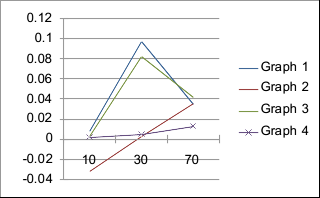
\includegraphics[width=\textwidth]{img/model_1run.png}
                \caption{Adj RAND}
                \label{fig:img/model_1run.png}
            \end{subfigure}
            \begin{subfigure}[b]{0.4\textwidth}
                \centering
                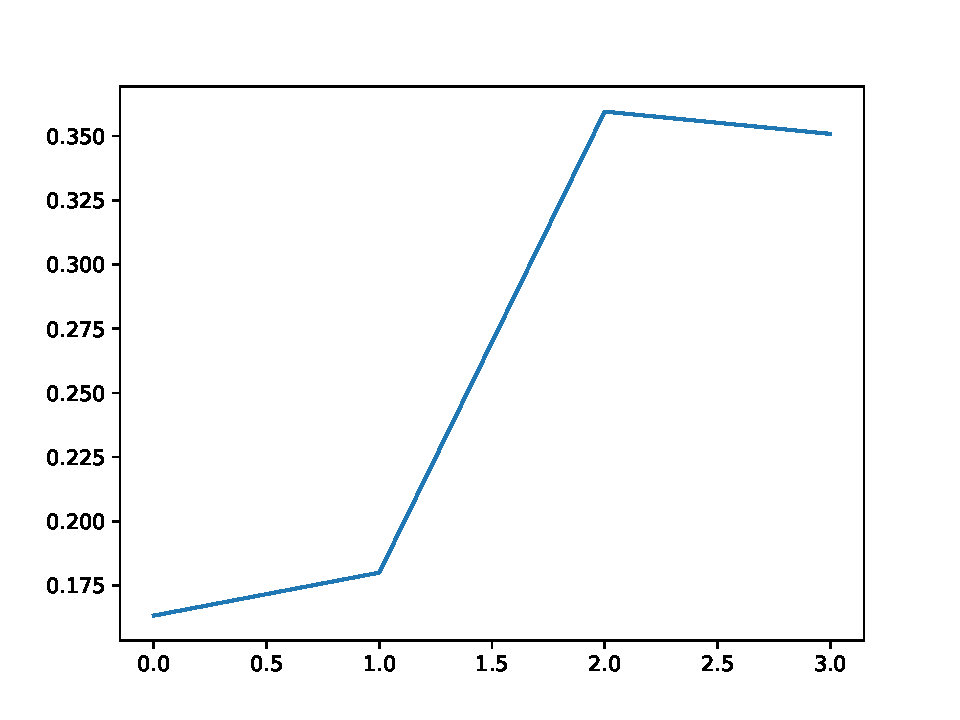
\includegraphics[width=\textwidth]{out/synthetic1/model1_scores1_40.pdf}
                \caption{Jaccard along iterations, for (Graph 1, 30)}
                \label{fig:}
            \end{subfigure}
        \end{center}
        \end{figure}
        
\end{frame}

\begin{frame}[c]
	\frametitle{Computing the score on the synthetic data (2)}
    Test 2: 2 communities have $n$ nodes, the other $n/4$, $\alpha = 0.2$.

    \begin{figure}
        \begin{center}
            \begin{subfigure}[b]{0.4\textwidth}
                \centering
                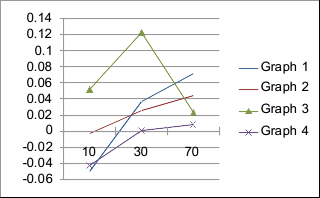
\includegraphics[width=\textwidth]{img/model_2run.png}
                \caption{Adj RAND}
                \label{fig:img/model_1run.png}
            \end{subfigure}
            \begin{subfigure}[b]{0.4\textwidth}
                \centering
                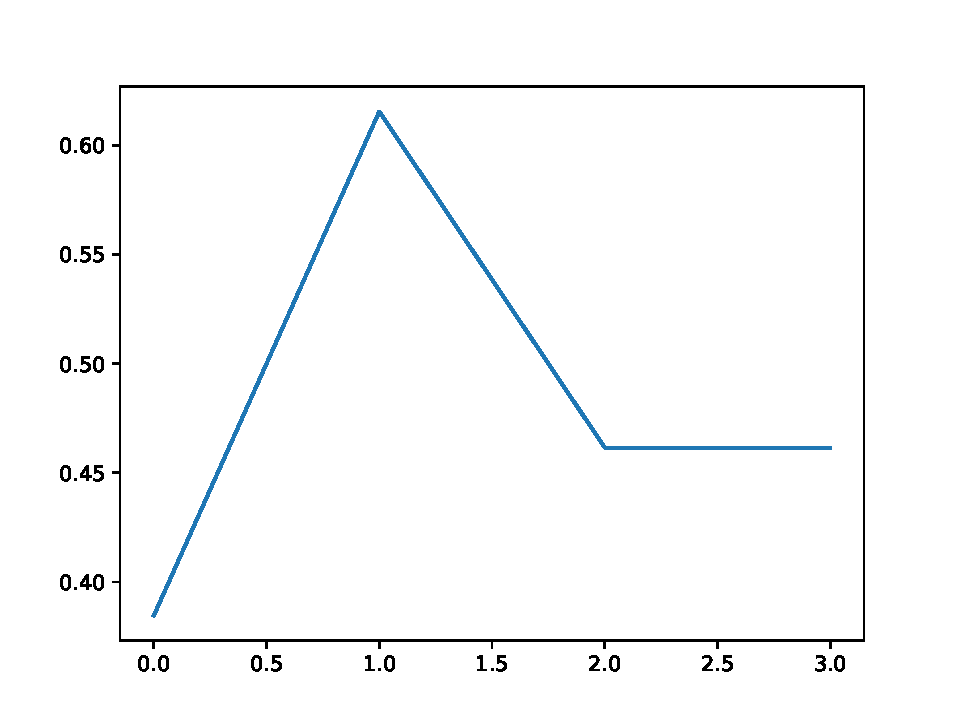
\includegraphics[width=\textwidth]{out/synthetic2/model1_scores6_10.pdf}
                \caption{Jaccard along iterations, for (Graph 3, 10)}
                \label{fig:}
            \end{subfigure}
        \end{center}
        \end{figure}
\end{frame}

\begin{frame}[c]
	\frametitle{Computing the score on the synthetic data (2)}
    Test 3: 2 communities have $n$ nodes, the other $n/4$, $\alpha$ chosen as
    the ratio of probability of negative edge over probability of edge inside
    the communities.

    \begin{figure}
        \begin{center}
            \begin{subfigure}[b]{0.4\textwidth}
                \centering
                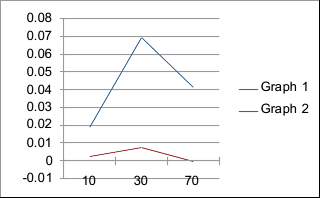
\includegraphics[width=\textwidth]{img/model_3run.png}
                \caption{Adj RAND}
                \label{fig:img/model_1run.png}
            \end{subfigure}
            \begin{subfigure}[b]{0.4\textwidth}
                \centering
                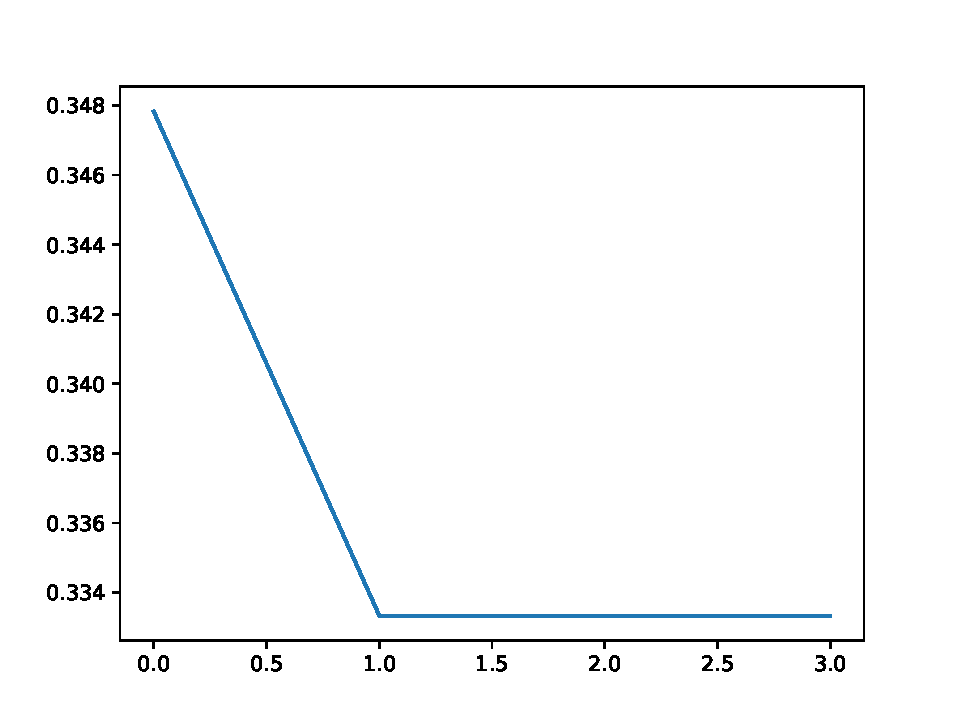
\includegraphics[width=\textwidth]{out/synthetic3/model1_scores0_10.pdf}
                \caption{Jaccard along iterations, for (Graph 1, 10)}
                \label{fig:}
            \end{subfigure}
        \end{center}
        \end{figure}
\end{frame}


% \begin{frame}[c]
%     \frametitle{Computing the score on the synthetic data (5)}
%     Third graph: much smaller distinction in the interaction between
%     communities.
%
%     \begin{figure}
%         \begin{center}
%             \begin{subfigure}[b]{0.3\textwidth}
%                 \centering
%                 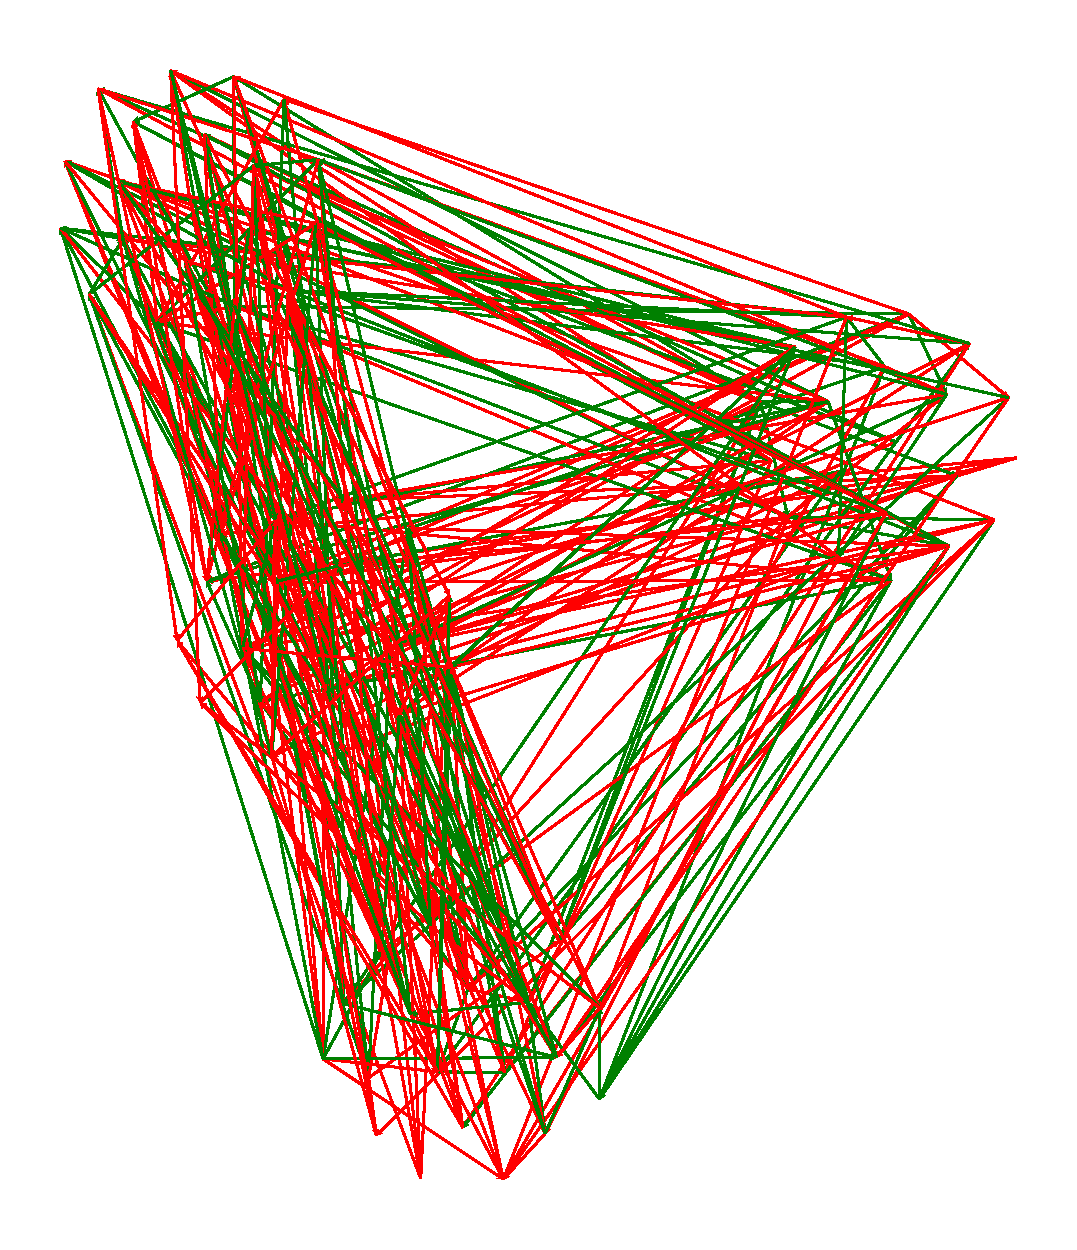
\includegraphics[width=\textwidth]{out/synthetic/model2_graph2.pdf}
%                 \caption{Graph}
%                 \label{fig:}
%             \end{subfigure}
%             \begin{subfigure}[b]{0.3\textwidth}
%                 \centering
%                 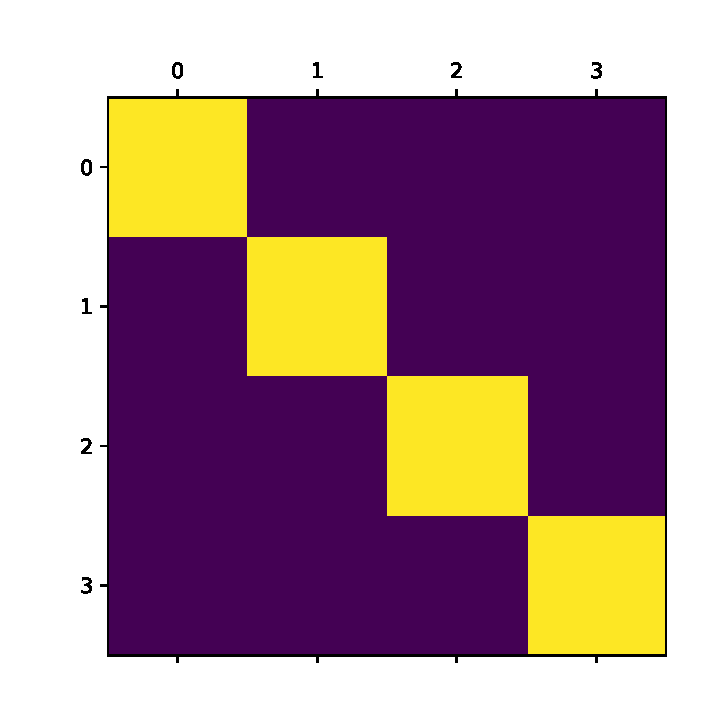
\includegraphics[width=\textwidth]{out/synthetic/model2_omega_positive3.pdf}
%                 \caption{$\omega ^{+} _{rs} $}
%                 \label{fig:out/synthetic/omega_positive1.pdf}
%             \end{subfigure}
%             \begin{subfigure}[b]{0.3\textwidth}
%                 \centering
%                 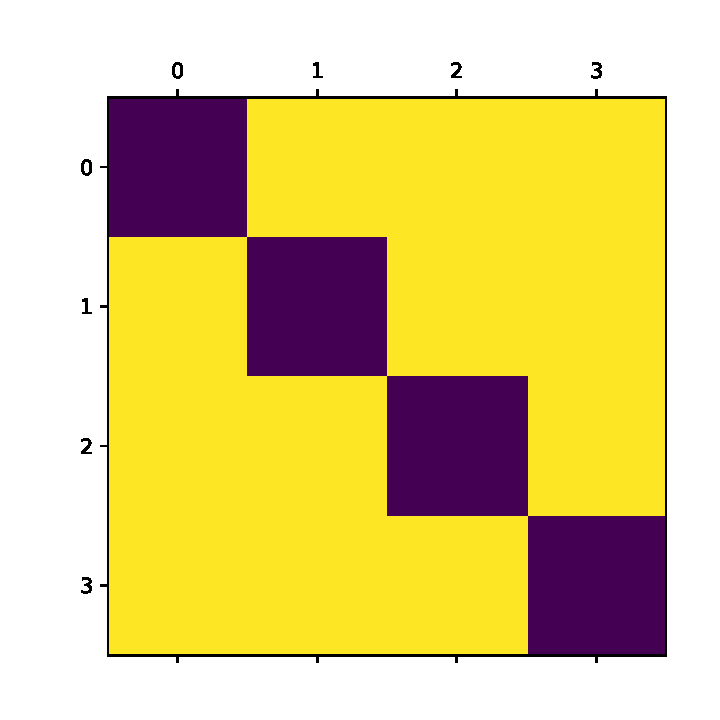
\includegraphics[width=\textwidth]{out/synthetic/model2_omega_negative3.pdf}
%                 \caption{$\omega ^{-} _{rs} $}
%                 \label{fig:}
%             \end{subfigure}
%         \end{center}
%     \end{figure}
%
%     $|V| = 80, \; |E| \approx 400, \; \eta(G) \approx 0.58, \; \bar{\xi}(G)
%         \approx 25$.
%
%     Rand $= 0.6$, adjusted Rand $= 0.007$
% \end{frame}

\begin{frame}[c]
	\frametitle{Observations on the result}
    Possible reasons for the poor results
	\begin{itemize}
        \item Solution of the Echo Chamber problem may find smaller groups of
            users inside the communities

        \item choice of $\alpha$
        \item results are also noisy due to the approximate algorithm
	\end{itemize}
\end{frame}



\end{document}
